% Chapter 1
% Delete this content and replace it with your own
% ------------------------------------------------------------------------------
\chapter{Analysis, Modeling, and Results} % enter the name of the chapter here
\label{cha:data} % enter the chapter label here (for cross-referencing)

Let us now go over what data we possess, what we did with this data, and how we came up with those results. 


\section{Analysis}
\label{sec:analysis}

We have gone over some key analyses in the chapter \ref{cha:novels-why}. Specifically, in the section \ref{sec:novels-list}. Thus, with this section, we shall directly be jumping into the data modeling, training/testing, and results section.

\subsection{Unique Character Sets}
\label{sec:unique-character-sets}

We have already defined the function above for cleaning up through coding in the section \ref{code:data-clean}. Thus, the same function can be imported and we can simply generate a couple of lists with unique characters of single and dual combinations. In the next part, we shall see how we could do it. 
\vspace{0.5cm}

\begin{code}
\label{code:data-split}
\begin{minted}[frame=single,framesep=10pt]{python}

all_characters = set()
dual_characters = set()

for file in all_files:
    
    book = open(PATH + file, 'r', encoding = 'utf-8-sig')
    novel = book.read()
    novel = data_cleaning(novel)

    #Single Characters
    all_characters |= set(novel)
    #Dual Characters
    dual_characters |= set(list(''.join(x) for x in zip(novel[:-1], novel[1:])))  

all_characters = sorted(list(all_characters))
dual_characters = sorted(list(dual_characters))
    
\end{minted}
\caption{Coding for generating small samples of single and dual character sets}.
\end{code}

\begin{figure}[H]
	\begin{center}
		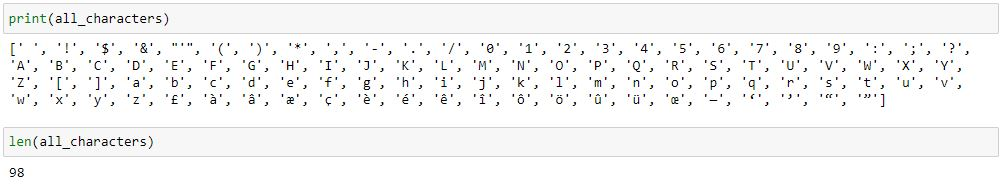
\includegraphics[width = 1.0\textwidth]{Images/single_chars.JPG} % enter the filename here
		\caption{Unique Individual Characters}
		\label{fig:single-chars-all}
	\end{center}
\end{figure}

\begin{figure}[H]
	\begin{center}
		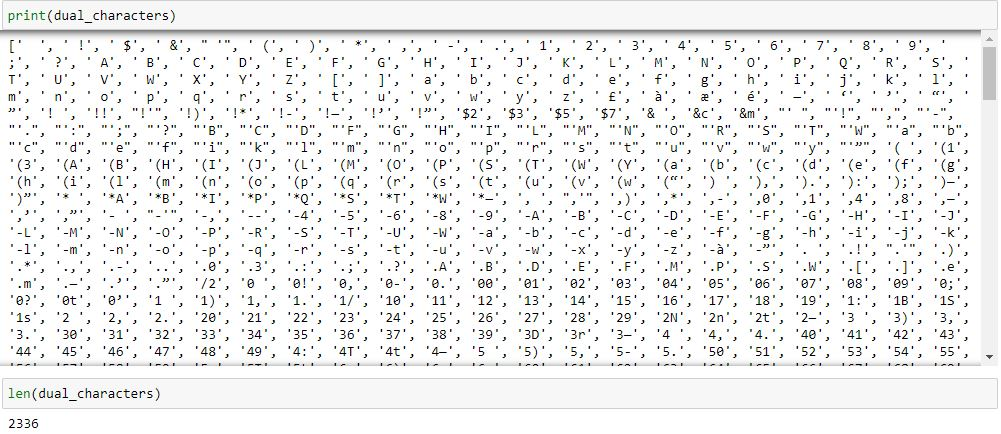
\includegraphics[width = 1.0\textwidth]{Images/dual_chars.JPG} % enter the filename here
		\caption{Unique Dual Character Sets}
		\label{fig:dual-chars-all}
	\end{center}
\end{figure}


\section{Modeling and Training}
\label{sec:modeling}

Now, we have already defined the libraries we would be using in the introduction \ref{sec:python-tools}. Now, let us continue with the overall structure and how we trained our model.
There will be 3 major tasks in this section.

\begin{itemize}
    \item Generating a list of unique single and dual character lists.
    \item Creating a probability distribution for single and dual character sets for each novel.
    \item Generate Log Probabilities and use the equations in \ref{sec:custom-bayes-implementation} into our model.
\end{itemize}
\vspace{0.5cm}

\begin{code}
\label{code:data-split}
\begin{minted}[frame=single,framesep=10pt]{python}
def data_split_custom(text):
    
    texts = len(text)
    # We are using a sample 80-20 train and test split for our novels. 
    split = int(0.8 * texts)
    return text[:split], text[split+1:]
\end{minted}
\caption{Our Function to Split our data into Train and Test samples for future use}.
\end{code}

\subsection{Log Probability Calculation}
\label{sec:log-probability-code}

In this section, we would be covering how we calculated individual and dual character probabilities for all the novels. In the first case of individual probabilities, a simple list works for each novel, yet however, for dual character probabilities, an n*n matrix, which is known as the Transition Matrix, mentioned in the section \label{sec:discrete-space-markov-chains}, and thus each of the novels would need their own DataFrames with these subsequent probabilities.

\subsubsection{Individual Probabilities}
\label{sec:individual-char-probs}
\vspace{0.5cm}

\begin{code}
\label{code:single-char-prob}
\begin{minted}[frame=single,framesep=10pt]{python}
probs = {}
probs_log = {}
charslen = {}

for file in all_files:
            
    book = open(PATH + file, 'r', encoding = 'utf-8-sig')       
    novel = book.read()
    novel = data_cleaning(novel)
    total_len = len(novel)
    novel_train, novel_test = data_split_custom(novel)
    
    probs[file] = {}
    probs_log[file] = {}
    charslen[file] = {}
    
    for char in all_characters:
        charcount = novel_train.count(char)
        probs[file][char] = charcount/total_len
        #Calculating Log Probabilities for all Novels over individual characters
        if charcount == 0:
            probs_log[file][char] = 0
        else:
            probs_log[file][char] = math.log((charcount)/(total_len))
probs_log_df = pd.DataFrame(probs_log)    
\end{minted}
\caption{Loop generates a DataFrame with Single Character Probabilities}.
\end{code}

With this, we get the following DataFrame, which lists out individual character probabilities within a novel. We have kept 0 as an actual occurrence to ensure dual character probabilities are distinguishable.

\begin{figure}[H]
	\begin{center}
		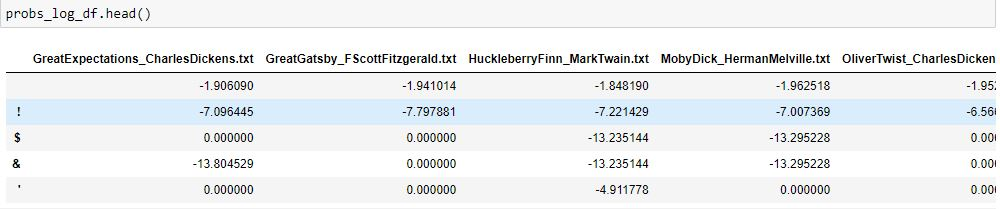
\includegraphics[width = 1.0\textwidth]{Images/single_char_probs.JPG} % enter the filename here
		\caption{Unique Single Character Matrix}
		\label{fig:single-char-prob-matrix}
	\end{center}
\end{figure}

\subsubsection{Dual Probabilities}
\label{sec:dual-char-probs}
\vspace{0.5cm}

\begin{code}
\label{code:transition-matrix}
\begin{minted}[frame=single,framesep=10pt]{python}
for file in all_files:
            
    book = open(PATH + file, 'r', encoding = 'utf-8-sig')
    novel = book.read()
    novel = data_cleaning(novel)
    novel_train, novel_test = data_split_custom(novel)
    counts = np.zeros((len(all_characters), len(all_characters)))
    pairs = zip(novel_train[:-1], novel_train[1:])
    
    for first, second in pairs:
        i = idx[first]
        j = idx[second]
        counts[i,j] += 1
    
    # Laplacian Smoothing
    counts += 1 
    
    #Defining a new DataFrame for each novel. 
    # As an example:
    # GreatExpectations_CharlesDickens is the count of co-occurrences of all characters
    # probs_GreatExpectations_CharlesDickens are the individual probabilities. 
    
    globals()[f"{file[:-4]}"] = counts
    mid_sum = np.sum(counts, axis=1)
    globals()[f"probs_{file[:-4]}"] = pd.DataFrame(counts/(mid_sum.reshape(len(mid_sum),1)), index = idx, columns = idx)
    globals()[f"logs_{file[:-4]}"] = pd.DataFrame(np.log(counts/(mid_sum.reshape(len(mid_sum),1))), index = idx, columns = idx)    
\end{minted}
\caption{Loop generates multiple DataFrames with Dual Character Probabilities}.
\end{code}

We learned about Laplacian Smoothing in the section \ref{sec:laplace-smoothing}. This is where it is extremely important to implement to avoid any data loss within dual character occurrences. The code \ref{code:transition-matrix} results in individual log and normal transition matrices. The names of each of the matrices are as follows. And after that, is an example of what the transition matrix for \textcite{great_expectations} would look like.

\begin{itemize}
    \item logs\textunderscore GreatExpectations\textunderscore CharlesDickens/ probs\textunderscore GreatExpectations\textunderscore CharlesDickens
    \item logs\textunderscore GreatGatsby\textunderscore FScottFitzgerald/ probs\textunderscore GreatGatsby\textunderscore FScottFitzgerald
    \item logs\textunderscore HuckleberryFinn\textunderscore MarkTwain/ probs\textunderscore HuckleberryFinn\textunderscore MarkTwain
    \item logs\textunderscore MobyDick\textunderscore HermanMelville/ probs\textunderscore MobyDick\textunderscore HermanMelville
    \item logs\textunderscore OliverTwist\textunderscore CharlesDickens/ probs\textunderscore OliverTwist\textunderscore CharlesDickens
    \item logs\textunderscore PridePrejudice\textunderscore JaneAusten/ probs\textunderscore PridePrejudice\textunderscore JaneAusten
    \item logs\textunderscore SherlockHolmes\textunderscore ArthurDoyle/ probs\textunderscore SherlockHolmes\textunderscore ArthurDoyle
    \item logs\textunderscore SignOfTheFour\textunderscore ArthurDoyle/ probs\textunderscore SignOfTheFour\textunderscore ArthurDoyle
\end{itemize}

\begin{figure}[H]
	\begin{center}
		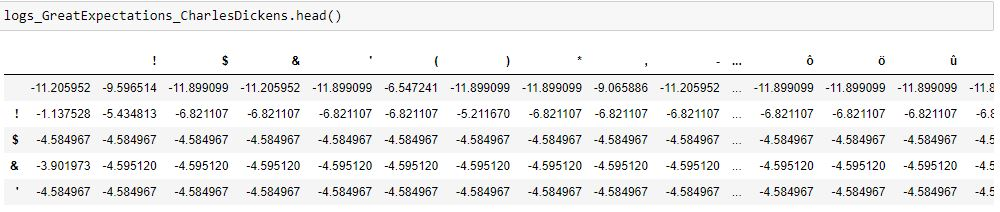
\includegraphics[width = 1.0\textwidth]{Images/transition_matrix.JPG} % enter the filename here
		\caption{Transition Matrix over Novels}
		\label{fig:dual-char-transition-matrix}
	\end{center}
\end{figure}

\textbf{Please Note: Since these are individual transition matrices, each novel in our dataset has a custom DataFrame. Now until this step, the entire code is reproducible over any given text and we can input any novels to generate it. However, the testing phase would be quite customized based on the testing text we choose, with further information in the section \ref{sec:results}}. 

\subsection{Custom Bayes' Rule Code}
\label{sec:code-custom-bayes-markov}

Now with this section, we shall finally implement the theory we studied and derived a final equation in the section \ref{sec:custom-bayes-implementation} with the derived equation \ref{eq:final_custom_bayes}.
\vspace{0.5cm}

\begin{code}
\label{code:final-custom-bayes}
\begin{minted}[frame=single,framesep=10pt]{python}
custom_MarkovChain = np.empty(len(all_files))
for i, file in enumerate(all_files):
    custom_MarkovChain[i] = probs_log_df[file].sum()
    
#With reducing the maximum of the entire model, we are regularizing the entire model.
custom_MarkovChain = custom_MarkovChain - custom_MarkovChain.max()

MarkovChain_Train = pd.DataFrame(data=custom_MarkovChain).T
MarkovChain_Train.columns=all_files    
\end{minted}
\caption{A 1*n DataFrame with final individual book log probabilities}.
\end{code}

With this, we get the following regularized log probabilities for each novel.

\begin{figure}[H]
	\begin{center}
		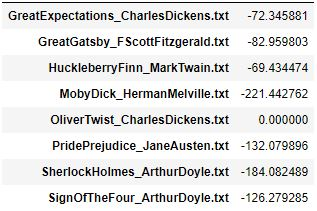
\includegraphics[width = 0.5\textwidth]{Images/markovchain_custom.JPG} % enter the filename here
		\caption{Markov Chain Probabilities}
		\label{fig:custom-markov-chain-probs-final}
	\end{center}
\end{figure}


\section{Testing and Results}
\label{sec:results}

Finally, when we go above and go through the code \ref{code:data-split}, there is a train and a test split. We use this function to create the test data set again, and then generate the log probabilities over the test data from our train data, predicting the closeness of authors with their actual work.

For our test, we shall only be focusing on two tests. It can be increased and changed by re-running the code, which shall be available on GitHub. 

Let us go over the process of testing our code. First, in order to test, we re-define the test pairs from the testing dataset. Please note, that there are way more efficient ways to perform this testing task, but since we are short on time, we are working with individual variables instead of a dynamic variable selection, as will be seen in the code 
\vspace{0.5cm}

\begin{code}
\label{code:testing-data-load}
\begin{minted}[frame=single,framesep=10pt]{python}
book = open(PATH + 'GreatExpectations_CharlesDickens.txt', 'r', encoding = 'utf-8-sig')
novel = book.read()
novel = data_cleaning(novel)
_, greatexp_test = data_split_custom(novel)

test_pairs = set(zip(greatexp_test[:-1], greatexp_test[1:]))
\end{minted}
\caption{Variable greatexp_test used for generating test set}.
\end{code}

Our test pairs look like this:

\begin{figure}[H]
	\begin{center}
		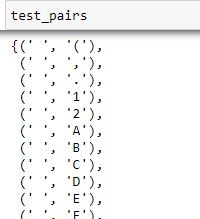
\includegraphics[width = 0.4\textwidth]{Images/test_pairs.JPG} % enter the filename here
		\caption{Test Dual Character Pairs}
		\label{fig:test-char-pairs}
	\end{center}
\end{figure}
\vspace{0.5cm}

\begin{code}
\label{code:testing-matrix-gen}
\begin{minted}[frame=single,framesep=10pt]{python}
#These variables are listed as abbreviations of the novel and the author name combined.
    
GECD_test = 0
GGFSF_test = 0
HFMT_test = 0
MDHM_test = 0
OTCD_test = 0
PPJA_test = 0
SAAD_test = 0
STFAD_test = 0

test_df = MarkovChain_Train.copy()

for first, second in test_pairs:
    
    GECD_test += logs_GreatExpectations_CharlesDickens.loc[first, second]
    GGFSF_test += logs_GreatGatsby_FScottFitzgerald.loc[first, second]
    HFMT_test += logs_HuckleberryFinn_MarkTwain.loc[first, second]
    MDHM_test += logs_MobyDick_HermanMelville.loc[first, second]
    OTCD_test += logs_OliverTwist_CharlesDickens.loc[first, second]
    PPJA_test += logs_PridePrejudice_JaneAusten.loc[first, second]
    SAAD_test += logs_SherlockHolmes_ArthurDoyle.loc[first, second]
    STFAD_test += logs_SignOfTheFour_ArthurDoyle.loc[first, second]

test_df['GreatExpectations_CharlesDickens.txt'] = GECD_test
test_df['GreatGatsby_FScottFitzgerald.txt'] = GGFSF_test
test_df['HuckleberryFinn_MarkTwain.txt'] = HFMT_test
test_df['MobyDick_HermanMelville.txt'] = MDHM_test
test_df['OliverTwist_CharlesDickens.txt'] = OTCD_test
test_df['PridePrejudice_JaneAusten.txt'] = PPJA_test
test_df['SherlockHolmes_ArthurDoyle.txt'] = SAAD_test
test_df['SignOfTheFour_ArthurDoyle.txt'] = STFAD_test

max_test_coef = max(GECD_test, GGFSF_test, HFMT_test, MDHM_test, OTCD_test, PPJA_test, SAAD_test, STFAD_test)

test_df = test_df - max_test_coef
test_df.T
\end{minted}
\caption{Semi-Reproducible Testing Process}.
\end{code}

When tested alongside with two books - \ref{sec:great-expectations} and \ref{sec:moby-dick}, give us some very interesting results. 

\begin{figure}[H]
	\begin{center}
		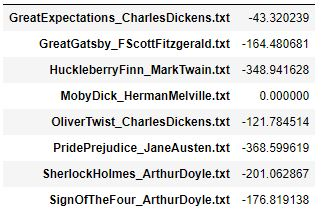
\includegraphics[width = 0.5\textwidth]{Images/testing_greatexp.JPG} % enter the filename here
		\caption{Great Expectations Testing Final Markov Chain Results}
		\label{fig:test-great-expectations}
	\end{center}
\end{figure}

\begin{figure}[H]
	\begin{center}
		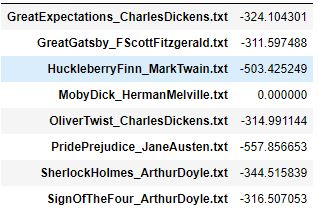
\includegraphics[width = 0.5\textwidth]{Images/testing_mobydick.JPG} % enter the filename here
		\caption{Moby Dick Testing Final Markov Chain Results}
		\label{fig:test-moby-dick}
	\end{center}
\end{figure}

Now, from \ref{fig:test-great-expectations}, we see that our model is predicting Great Expectations to be the second highest value. Moby Dick has the lowest value in the predicted value when we incorporate the equation \ref{eq:custom-test-results}. However, when we look at the prediction for Moby Dick, we get a very well-defined value whereas all other books are quite distant from the value for Moby Dick when it was trained over itself. However, this is just the first iteration, and in case we began training the model over a Gradient Descent model, in order to reduce the probabilities over a given sequence, we could have observed better results. But since we do not train over Markov Chains, this first iteration also gives us very good results.

We shall conclude our dissertation in the next chapter.

